% Created by tikzDevice version 0.12.3.1 on 2022-09-05 08:11:25
% !TEX encoding = UTF-8 Unicode
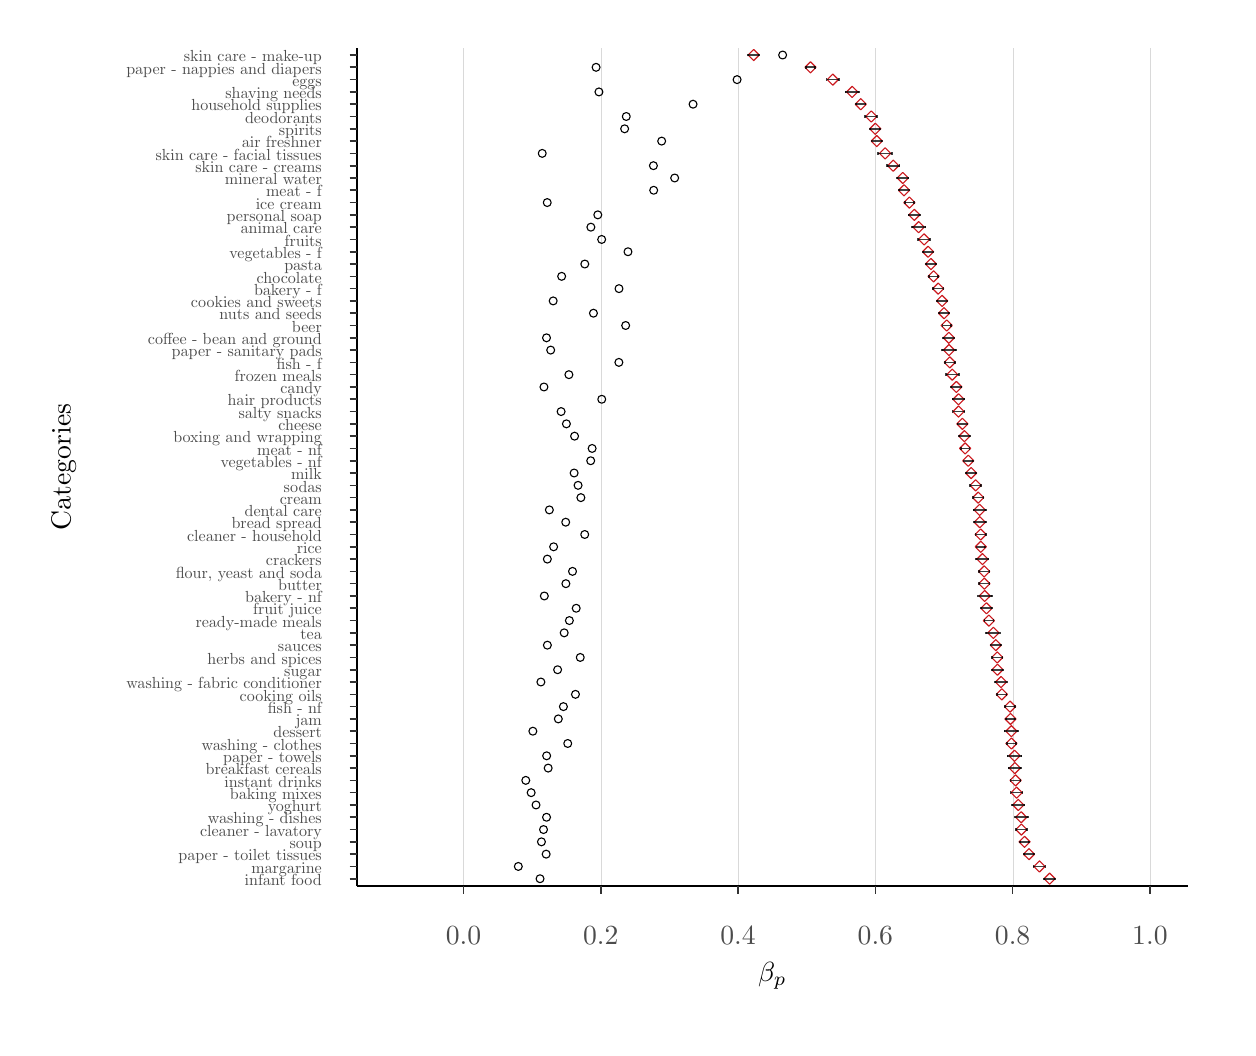
\begin{tikzpicture}[x=1pt,y=1pt]
\definecolor{fillColor}{RGB}{255,255,255}
\path[use as bounding box,fill=fillColor,fill opacity=0.00] (0,0) rectangle (433.62,361.35);
\begin{scope}
\path[clip] (  0.00,  0.00) rectangle (433.62,361.35);
\definecolor{drawColor}{RGB}{255,255,255}
\definecolor{fillColor}{RGB}{255,255,255}

\path[draw=drawColor,line width= 0.6pt,line join=round,line cap=round,fill=fillColor] (  0.00,  0.00) rectangle (433.62,361.35);
\end{scope}
\begin{scope}
\path[clip] (119.04, 51.15) rectangle (419.17,354.12);
\definecolor{drawColor}{RGB}{255,255,255}

\path[draw=drawColor,line width= 0.3pt,line join=round] (132.68, 51.15) --
	(132.68,354.12);

\path[draw=drawColor,line width= 0.3pt,line join=round] (182.29, 51.15) --
	(182.29,354.12);

\path[draw=drawColor,line width= 0.3pt,line join=round] (231.90, 51.15) --
	(231.90,354.12);

\path[draw=drawColor,line width= 0.3pt,line join=round] (281.51, 51.15) --
	(281.51,354.12);

\path[draw=drawColor,line width= 0.3pt,line join=round] (331.11, 51.15) --
	(331.11,354.12);

\path[draw=drawColor,line width= 0.3pt,line join=round] (380.72, 51.15) --
	(380.72,354.12);
\definecolor{drawColor}{gray}{0.85}

\path[draw=drawColor,line width= 0.1pt,line join=round] (157.49, 51.15) --
	(157.49,354.12);

\path[draw=drawColor,line width= 0.1pt,line join=round] (207.09, 51.15) --
	(207.09,354.12);

\path[draw=drawColor,line width= 0.1pt,line join=round] (256.70, 51.15) --
	(256.70,354.12);

\path[draw=drawColor,line width= 0.1pt,line join=round] (306.31, 51.15) --
	(306.31,354.12);

\path[draw=drawColor,line width= 0.1pt,line join=round] (355.92, 51.15) --
	(355.92,354.12);

\path[draw=drawColor,line width= 0.1pt,line join=round] (405.52, 51.15) --
	(405.52,354.12);
\definecolor{drawColor}{RGB}{0,0,0}

\path[draw=drawColor,line width= 0.4pt,line join=round,line cap=round] (229.09,320.36) circle (  1.43);

\path[draw=drawColor,line width= 0.4pt,line join=round,line cap=round] (203.51,289.26) circle (  1.43);

\path[draw=drawColor,line width= 0.4pt,line join=round,line cap=round] (213.67,267.05) circle (  1.43);

\path[draw=drawColor,line width= 0.4pt,line join=round,line cap=round] (186.69,155.99) circle (  1.43);

\path[draw=drawColor,line width= 0.4pt,line join=round,line cap=round] (181.93, 84.92) circle (  1.43);

\path[draw=drawColor,line width= 0.4pt,line join=round,line cap=round] (216.08,253.73) circle (  1.43);

\path[draw=drawColor,line width= 0.4pt,line join=round,line cap=round] (197.62,213.74) circle (  1.43);

\path[draw=drawColor,line width= 0.4pt,line join=round,line cap=round] (194.42,182.65) circle (  1.43);

\path[draw=drawColor,line width= 0.4pt,line join=round,line cap=round] (188.08, 93.80) circle (  1.43);

\path[draw=drawColor,line width= 0.4pt,line join=round,line cap=round] (194.48,160.44) circle (  1.43);

\path[draw=drawColor,line width= 0.4pt,line join=round,line cap=round] (186.56,231.51) circle (  1.43);

\path[draw=drawColor,line width= 0.4pt,line join=round,line cap=round] (194.67,218.19) circle (  1.43);

\path[draw=drawColor,line width= 0.4pt,line join=round,line cap=round] (192.95,271.49) circle (  1.43);

\path[draw=drawColor,line width= 0.4pt,line join=round,line cap=round] (201.29,178.21) circle (  1.43);

\path[draw=drawColor,line width= 0.4pt,line join=round,line cap=round] (186.40, 71.59) circle (  1.43);

\path[draw=drawColor,line width= 0.4pt,line join=round,line cap=round] (187.48,249.28) circle (  1.43);

\path[draw=drawColor,line width= 0.4pt,line join=round,line cap=round] (189.89,262.61) circle (  1.43);

\path[draw=drawColor,line width= 0.4pt,line join=round,line cap=round] (197.94,120.45) circle (  1.43);

\path[draw=drawColor,line width= 0.4pt,line join=round,line cap=round] (187.78,169.32) circle (  1.43);

\path[draw=drawColor,line width= 0.4pt,line join=round,line cap=round] (199.90,191.53) circle (  1.43);

\path[draw=drawColor,line width= 0.4pt,line join=round,line cap=round] (188.51,187.09) circle (  1.43);

\path[draw=drawColor,line width= 0.4pt,line join=round,line cap=round] (216.30,329.25) circle (  1.43);

\path[draw=drawColor,line width= 0.4pt,line join=round,line cap=round] (182.55,107.13) circle (  1.43);

\path[draw=drawColor,line width= 0.4pt,line join=round,line cap=round] (256.34,342.57) circle (  1.43);

\path[draw=drawColor,line width= 0.4pt,line join=round,line cap=round] (213.63,240.40) circle (  1.43);

\path[draw=drawColor,line width= 0.4pt,line join=round,line cap=round] (193.59,116.01) circle (  1.43);

\path[draw=drawColor,line width= 0.4pt,line join=round,line cap=round] (196.88,164.88) circle (  1.43);

\path[draw=drawColor,line width= 0.4pt,line join=round,line cap=round] (195.57,235.96) circle (  1.43);

\path[draw=drawColor,line width= 0.4pt,line join=round,line cap=round] (198.21,151.55) circle (  1.43);

\path[draw=drawColor,line width= 0.4pt,line join=round,line cap=round] (207.41,284.82) circle (  1.43);

\path[draw=drawColor,line width= 0.4pt,line join=round,line cap=round] (207.44,227.07) circle (  1.43);

\path[draw=drawColor,line width= 0.4pt,line join=round,line cap=round] (199.67,133.78) circle (  1.43);

\path[draw=drawColor,line width= 0.4pt,line join=round,line cap=round] (240.43,333.69) circle (  1.43);

\path[draw=drawColor,line width= 0.4pt,line join=round,line cap=round] (187.74,298.15) circle (  1.43);

\path[draw=drawColor,line width= 0.4pt,line join=round,line cap=round] (185.14, 53.82) circle (  1.43);

\path[draw=drawColor,line width= 0.4pt,line join=round,line cap=round] (179.99, 89.36) circle (  1.43);

\path[draw=drawColor,line width= 0.4pt,line join=round,line cap=round] (191.74,111.57) circle (  1.43);

\path[draw=drawColor,line width= 0.4pt,line join=round,line cap=round] (177.29, 58.26) circle (  1.43);

\path[draw=drawColor,line width= 0.4pt,line join=round,line cap=round] (226.21,302.59) circle (  1.43);

\path[draw=drawColor,line width= 0.4pt,line join=round,line cap=round] (203.96,209.30) circle (  1.43);

\path[draw=drawColor,line width= 0.4pt,line join=round,line cap=round] (197.46,200.42) circle (  1.43);

\path[draw=drawColor,line width= 0.4pt,line join=round,line cap=round] (233.79,307.03) circle (  1.43);

\path[draw=drawColor,line width= 0.4pt,line join=round,line cap=round] (204.44,258.17) circle (  1.43);

\path[draw=drawColor,line width= 0.4pt,line join=round,line cap=round] (205.39,347.02) circle (  1.43);

\path[draw=drawColor,line width= 0.4pt,line join=round,line cap=round] (188.99,244.84) circle (  1.43);

\path[draw=drawColor,line width= 0.4pt,line join=round,line cap=round] (187.35, 62.70) circle (  1.43);

\path[draw=drawColor,line width= 0.4pt,line join=round,line cap=round] (187.53, 98.24) circle (  1.43);

\path[draw=drawColor,line width= 0.4pt,line join=round,line cap=round] (201.31,275.94) circle (  1.43);

\path[draw=drawColor,line width= 0.4pt,line join=round,line cap=round] (206.01,293.71) circle (  1.43);

\path[draw=drawColor,line width= 0.4pt,line join=round,line cap=round] (195.74,147.11) circle (  1.43);

\path[draw=drawColor,line width= 0.4pt,line join=round,line cap=round] (190.05,173.76) circle (  1.43);

\path[draw=drawColor,line width= 0.4pt,line join=round,line cap=round] (192.75,222.63) circle (  1.43);

\path[draw=drawColor,line width= 0.4pt,line join=round,line cap=round] (187.79,138.22) circle (  1.43);

\path[draw=drawColor,line width= 0.4pt,line join=round,line cap=round] (206.43,338.13) circle (  1.43);

\path[draw=drawColor,line width= 0.4pt,line join=round,line cap=round] (226.11,311.48) circle (  1.43);

\path[draw=drawColor,line width= 0.4pt,line join=round,line cap=round] (185.93,315.92) circle (  1.43);

\path[draw=drawColor,line width= 0.4pt,line join=round,line cap=round] (272.80,351.46) circle (  1.43);

\path[draw=drawColor,line width= 0.4pt,line join=round,line cap=round] (198.88,195.97) circle (  1.43);

\path[draw=drawColor,line width= 0.4pt,line join=round,line cap=round] (185.65, 67.15) circle (  1.43);

\path[draw=drawColor,line width= 0.4pt,line join=round,line cap=round] (215.71,324.80) circle (  1.43);

\path[draw=drawColor,line width= 0.4pt,line join=round,line cap=round] (191.49,129.34) circle (  1.43);

\path[draw=drawColor,line width= 0.4pt,line join=round,line cap=round] (193.87,142.67) circle (  1.43);

\path[draw=drawColor,line width= 0.4pt,line join=round,line cap=round] (216.92,280.38) circle (  1.43);

\path[draw=drawColor,line width= 0.4pt,line join=round,line cap=round] (203.45,204.86) circle (  1.43);

\path[draw=drawColor,line width= 0.4pt,line join=round,line cap=round] (195.15,102.69) circle (  1.43);

\path[draw=drawColor,line width= 0.4pt,line join=round,line cap=round] (187.49, 76.03) circle (  1.43);

\path[draw=drawColor,line width= 0.4pt,line join=round,line cap=round] (185.45,124.90) circle (  1.43);

\path[draw=drawColor,line width= 0.4pt,line join=round,line cap=round] (183.69, 80.47) circle (  1.43);
\definecolor{drawColor}{RGB}{203,24,29}

\path[draw=drawColor,line width= 0.4pt,line join=round,line cap=round] (304.79,320.36) --
	(306.81,322.38) --
	(308.83,320.36) --
	(306.81,318.34) --
	cycle;

\path[draw=drawColor,line width= 0.4pt,line join=round,line cap=round] (319.93,289.26) --
	(321.95,291.28) --
	(323.97,289.26) --
	(321.95,287.25) --
	cycle;

\path[draw=drawColor,line width= 0.4pt,line join=round,line cap=round] (326.99,267.05) --
	(329.01,269.07) --
	(331.02,267.05) --
	(329.01,265.04) --
	cycle;

\path[draw=drawColor,line width= 0.4pt,line join=round,line cap=round] (343.78,155.99) --
	(345.80,158.01) --
	(347.82,155.99) --
	(345.80,153.98) --
	cycle;

\path[draw=drawColor,line width= 0.4pt,line join=round,line cap=round] (355.34, 84.92) --
	(357.35, 86.93) --
	(359.37, 84.92) --
	(357.35, 82.90) --
	cycle;

\path[draw=drawColor,line width= 0.4pt,line join=round,line cap=round] (330.07,253.73) --
	(332.09,255.74) --
	(334.10,253.73) --
	(332.09,251.71) --
	cycle;

\path[draw=drawColor,line width= 0.4pt,line join=round,line cap=round] (336.47,213.74) --
	(338.49,215.76) --
	(340.51,213.74) --
	(338.49,211.73) --
	cycle;

\path[draw=drawColor,line width= 0.4pt,line join=round,line cap=round] (342.03,182.65) --
	(344.05,184.67) --
	(346.06,182.65) --
	(344.05,180.63) --
	cycle;

\path[draw=drawColor,line width= 0.4pt,line join=round,line cap=round] (354.68, 93.80) --
	(356.69, 95.82) --
	(358.71, 93.80) --
	(356.69, 91.78) --
	cycle;

\path[draw=drawColor,line width= 0.4pt,line join=round,line cap=round] (343.66,160.44) --
	(345.68,162.45) --
	(347.70,160.44) --
	(345.68,158.42) --
	cycle;

\path[draw=drawColor,line width= 0.4pt,line join=round,line cap=round] (333.56,231.51) --
	(335.58,233.53) --
	(337.60,231.51) --
	(335.58,229.50) --
	cycle;

\path[draw=drawColor,line width= 0.4pt,line join=round,line cap=round] (335.76,218.19) --
	(337.77,220.20) --
	(339.79,218.19) --
	(337.77,216.17) --
	cycle;

\path[draw=drawColor,line width= 0.4pt,line join=round,line cap=round] (325.32,271.49) --
	(327.34,273.51) --
	(329.36,271.49) --
	(327.34,269.48) --
	cycle;

\path[draw=drawColor,line width= 0.4pt,line join=round,line cap=round] (342.34,178.21) --
	(344.35,180.22) --
	(346.37,178.21) --
	(344.35,176.19) --
	cycle;

\path[draw=drawColor,line width= 0.4pt,line join=round,line cap=round] (357.06, 71.59) --
	(359.07, 73.61) --
	(361.09, 71.59) --
	(359.07, 69.57) --
	cycle;

\path[draw=drawColor,line width= 0.4pt,line join=round,line cap=round] (330.85,249.28) --
	(332.86,251.30) --
	(334.88,249.28) --
	(332.86,247.27) --
	cycle;

\path[draw=drawColor,line width= 0.4pt,line join=round,line cap=round] (328.40,262.61) --
	(330.41,264.63) --
	(332.43,262.61) --
	(330.41,260.59) --
	cycle;

\path[draw=drawColor,line width= 0.4pt,line join=round,line cap=round] (349.99,120.45) --
	(352.01,122.47) --
	(354.03,120.45) --
	(352.01,118.44) --
	cycle;

\path[draw=drawColor,line width= 0.4pt,line join=round,line cap=round] (342.99,169.32) --
	(345.01,171.34) --
	(347.02,169.32) --
	(345.01,167.30) --
	cycle;

\path[draw=drawColor,line width= 0.4pt,line join=round,line cap=round] (341.46,191.53) --
	(343.48,193.55) --
	(345.50,191.53) --
	(343.48,189.51) --
	cycle;

\path[draw=drawColor,line width= 0.4pt,line join=round,line cap=round] (341.96,187.09) --
	(343.98,189.11) --
	(346.00,187.09) --
	(343.98,185.07) --
	cycle;

\path[draw=drawColor,line width= 0.4pt,line join=round,line cap=round] (302.80,329.25) --
	(304.82,331.26) --
	(306.84,329.25) --
	(304.82,327.23) --
	cycle;

\path[draw=drawColor,line width= 0.4pt,line join=round,line cap=round] (353.43,107.13) --
	(355.45,109.14) --
	(357.46,107.13) --
	(355.45,105.11) --
	cycle;

\path[draw=drawColor,line width= 0.4pt,line join=round,line cap=round] (288.90,342.57) --
	(290.92,344.59) --
	(292.94,342.57) --
	(290.92,340.56) --
	cycle;

\path[draw=drawColor,line width= 0.4pt,line join=round,line cap=round] (331.18,240.40) --
	(333.20,242.42) --
	(335.22,240.40) --
	(333.20,238.38) --
	cycle;

\path[draw=drawColor,line width= 0.4pt,line join=round,line cap=round] (352.96,116.01) --
	(354.97,118.03) --
	(356.99,116.01) --
	(354.97,113.99) --
	cycle;

\path[draw=drawColor,line width= 0.4pt,line join=round,line cap=round] (343.61,164.88) --
	(345.63,166.90) --
	(347.65,164.88) --
	(345.63,162.86) --
	cycle;

\path[draw=drawColor,line width= 0.4pt,line join=round,line cap=round] (332.08,235.96) --
	(334.10,237.97) --
	(336.11,235.96) --
	(334.10,233.94) --
	cycle;

\path[draw=drawColor,line width= 0.4pt,line join=round,line cap=round] (344.44,151.55) --
	(346.45,153.57) --
	(348.47,151.55) --
	(346.45,149.53) --
	cycle;

\path[draw=drawColor,line width= 0.4pt,line join=round,line cap=round] (321.90,284.82) --
	(323.92,286.84) --
	(325.94,284.82) --
	(323.92,282.80) --
	cycle;

\path[draw=drawColor,line width= 0.4pt,line join=round,line cap=round] (334.35,227.07) --
	(336.37,229.09) --
	(338.39,227.07) --
	(336.37,225.05) --
	cycle;

\path[draw=drawColor,line width= 0.4pt,line join=round,line cap=round] (348.33,133.78) --
	(350.35,135.80) --
	(352.36,133.78) --
	(350.35,131.76) --
	cycle;

\path[draw=drawColor,line width= 0.4pt,line join=round,line cap=round] (299.02,333.69) --
	(301.03,335.71) --
	(303.05,333.69) --
	(301.03,331.67) --
	cycle;

\path[draw=drawColor,line width= 0.4pt,line join=round,line cap=round] (316.59,298.15) --
	(318.61,300.17) --
	(320.62,298.15) --
	(318.61,296.13) --
	cycle;

\path[draw=drawColor,line width= 0.4pt,line join=round,line cap=round] (367.26, 53.82) --
	(369.27, 55.84) --
	(371.29, 53.82) --
	(369.27, 51.80) --
	cycle;

\path[draw=drawColor,line width= 0.4pt,line join=round,line cap=round] (354.95, 89.36) --
	(356.97, 91.38) --
	(358.98, 89.36) --
	(356.97, 87.34) --
	cycle;

\path[draw=drawColor,line width= 0.4pt,line join=round,line cap=round] (353.11,111.57) --
	(355.13,113.59) --
	(357.15,111.57) --
	(355.13,109.55) --
	cycle;

\path[draw=drawColor,line width= 0.4pt,line join=round,line cap=round] (363.58, 58.26) --
	(365.60, 60.28) --
	(367.62, 58.26) --
	(365.60, 56.24) --
	cycle;

\path[draw=drawColor,line width= 0.4pt,line join=round,line cap=round] (314.66,302.59) --
	(316.68,304.61) --
	(318.70,302.59) --
	(316.68,300.57) --
	cycle;

\path[draw=drawColor,line width= 0.4pt,line join=round,line cap=round] (336.72,209.30) --
	(338.74,211.32) --
	(340.75,209.30) --
	(338.74,207.28) --
	cycle;

\path[draw=drawColor,line width= 0.4pt,line join=round,line cap=round] (338.89,200.42) --
	(340.91,202.43) --
	(342.93,200.42) --
	(340.91,198.40) --
	cycle;

\path[draw=drawColor,line width= 0.4pt,line join=round,line cap=round] (314.20,307.03) --
	(316.22,309.05) --
	(318.24,307.03) --
	(316.22,305.02) --
	cycle;

\path[draw=drawColor,line width= 0.4pt,line join=round,line cap=round] (329.10,258.17) --
	(331.12,260.19) --
	(333.13,258.17) --
	(331.12,256.15) --
	cycle;

\path[draw=drawColor,line width= 0.4pt,line join=round,line cap=round] (280.85,347.02) --
	(282.86,349.03) --
	(284.88,347.02) --
	(282.86,345.00) --
	cycle;

\path[draw=drawColor,line width= 0.4pt,line join=round,line cap=round] (330.90,244.84) --
	(332.92,246.86) --
	(334.94,244.84) --
	(332.92,242.82) --
	cycle;

\path[draw=drawColor,line width= 0.4pt,line join=round,line cap=round] (359.81, 62.70) --
	(361.83, 64.72) --
	(363.85, 62.70) --
	(361.83, 60.69) --
	cycle;

\path[draw=drawColor,line width= 0.4pt,line join=round,line cap=round] (354.57, 98.24) --
	(356.59,100.26) --
	(358.61, 98.24) --
	(356.59, 96.23) --
	cycle;

\path[draw=drawColor,line width= 0.4pt,line join=round,line cap=round] (324.38,275.94) --
	(326.40,277.95) --
	(328.42,275.94) --
	(326.40,273.92) --
	cycle;

\path[draw=drawColor,line width= 0.4pt,line join=round,line cap=round] (318.36,293.71) --
	(320.38,295.72) --
	(322.40,293.71) --
	(320.38,291.69) --
	cycle;

\path[draw=drawColor,line width= 0.4pt,line join=round,line cap=round] (345.31,147.11) --
	(347.33,149.13) --
	(349.35,147.11) --
	(347.33,145.09) --
	cycle;

\path[draw=drawColor,line width= 0.4pt,line join=round,line cap=round] (342.39,173.76) --
	(344.40,175.78) --
	(346.42,173.76) --
	(344.40,171.75) --
	cycle;

\path[draw=drawColor,line width= 0.4pt,line join=round,line cap=round] (334.35,222.63) --
	(336.37,224.65) --
	(338.39,222.63) --
	(336.37,220.61) --
	cycle;

\path[draw=drawColor,line width= 0.4pt,line join=round,line cap=round] (347.80,138.22) --
	(349.82,140.24) --
	(351.83,138.22) --
	(349.82,136.21) --
	cycle;

\path[draw=drawColor,line width= 0.4pt,line join=round,line cap=round] (295.92,338.13) --
	(297.93,340.15) --
	(299.95,338.13) --
	(297.93,336.11) --
	cycle;

\path[draw=drawColor,line width= 0.4pt,line join=round,line cap=round] (310.74,311.48) --
	(312.76,313.49) --
	(314.78,311.48) --
	(312.76,309.46) --
	cycle;

\path[draw=drawColor,line width= 0.4pt,line join=round,line cap=round] (307.80,315.92) --
	(309.82,317.94) --
	(311.84,315.92) --
	(309.82,313.90) --
	cycle;

\path[draw=drawColor,line width= 0.4pt,line join=round,line cap=round] (260.32,351.46) --
	(262.33,353.48) --
	(264.35,351.46) --
	(262.33,349.44) --
	cycle;

\path[draw=drawColor,line width= 0.4pt,line join=round,line cap=round] (340.53,195.97) --
	(342.55,197.99) --
	(344.57,195.97) --
	(342.55,193.96) --
	cycle;

\path[draw=drawColor,line width= 0.4pt,line join=round,line cap=round] (358.19, 67.15) --
	(360.21, 69.16) --
	(362.23, 67.15) --
	(360.21, 65.13) --
	cycle;

\path[draw=drawColor,line width= 0.4pt,line join=round,line cap=round] (304.26,324.80) --
	(306.28,326.82) --
	(308.30,324.80) --
	(306.28,322.79) --
	cycle;

\path[draw=drawColor,line width= 0.4pt,line join=round,line cap=round] (348.41,129.34) --
	(350.42,131.36) --
	(352.44,129.34) --
	(350.42,127.32) --
	cycle;

\path[draw=drawColor,line width= 0.4pt,line join=round,line cap=round] (346.94,142.67) --
	(348.96,144.68) --
	(350.97,142.67) --
	(348.96,140.65) --
	cycle;

\path[draw=drawColor,line width= 0.4pt,line join=round,line cap=round] (323.34,280.38) --
	(325.36,282.40) --
	(327.38,280.38) --
	(325.36,278.36) --
	cycle;

\path[draw=drawColor,line width= 0.4pt,line join=round,line cap=round] (337.85,204.86) --
	(339.86,206.88) --
	(341.88,204.86) --
	(339.86,202.84) --
	cycle;

\path[draw=drawColor,line width= 0.4pt,line join=round,line cap=round] (353.45,102.69) --
	(355.47,104.70) --
	(357.48,102.69) --
	(355.47,100.67) --
	cycle;

\path[draw=drawColor,line width= 0.4pt,line join=round,line cap=round] (356.97, 76.03) --
	(358.99, 78.05) --
	(361.00, 76.03) --
	(358.99, 74.01) --
	cycle;

\path[draw=drawColor,line width= 0.4pt,line join=round,line cap=round] (349.71,124.90) --
	(351.72,126.91) --
	(353.74,124.90) --
	(351.72,122.88) --
	cycle;

\path[draw=drawColor,line width= 0.4pt,line join=round,line cap=round] (355.93, 80.47) --
	(357.95, 82.49) --
	(359.96, 80.47) --
	(357.95, 78.46) --
	cycle;
\definecolor{drawColor}{RGB}{0,0,0}

\path[draw=drawColor,draw opacity=0.75,line width= 0.6pt,line join=round] (308.66,319.92) --
	(308.66,320.81);

\path[draw=drawColor,draw opacity=0.75,line width= 0.6pt,line join=round] (308.66,320.36) --
	(304.96,320.36);

\path[draw=drawColor,draw opacity=0.75,line width= 0.6pt,line join=round] (304.96,319.92) --
	(304.96,320.81);

\path[draw=drawColor,draw opacity=0.75,line width= 0.6pt,line join=round] (324.45,288.82) --
	(324.45,289.71);

\path[draw=drawColor,draw opacity=0.75,line width= 0.6pt,line join=round] (324.45,289.26) --
	(319.45,289.26);

\path[draw=drawColor,draw opacity=0.75,line width= 0.6pt,line join=round] (319.45,288.82) --
	(319.45,289.71);

\path[draw=drawColor,draw opacity=0.75,line width= 0.6pt,line join=round] (330.87,266.61) --
	(330.87,267.50);

\path[draw=drawColor,draw opacity=0.75,line width= 0.6pt,line join=round] (330.87,267.05) --
	(327.14,267.05);

\path[draw=drawColor,draw opacity=0.75,line width= 0.6pt,line join=round] (327.14,266.61) --
	(327.14,267.50);

\path[draw=drawColor,draw opacity=0.75,line width= 0.6pt,line join=round] (348.34,155.55) --
	(348.34,156.44);

\path[draw=drawColor,draw opacity=0.75,line width= 0.6pt,line join=round] (348.34,155.99) --
	(343.25,155.99);

\path[draw=drawColor,draw opacity=0.75,line width= 0.6pt,line join=round] (343.25,155.55) --
	(343.25,156.44);

\path[draw=drawColor,draw opacity=0.75,line width= 0.6pt,line join=round] (359.53, 84.47) --
	(359.53, 85.36);

\path[draw=drawColor,draw opacity=0.75,line width= 0.6pt,line join=round] (359.53, 84.92) --
	(355.18, 84.92);

\path[draw=drawColor,draw opacity=0.75,line width= 0.6pt,line join=round] (355.18, 84.47) --
	(355.18, 85.36);

\path[draw=drawColor,draw opacity=0.75,line width= 0.6pt,line join=round] (333.61,253.28) --
	(333.61,254.17);

\path[draw=drawColor,draw opacity=0.75,line width= 0.6pt,line join=round] (333.61,253.73) --
	(330.57,253.73);

\path[draw=drawColor,draw opacity=0.75,line width= 0.6pt,line join=round] (330.57,253.28) --
	(330.57,254.17);

\path[draw=drawColor,draw opacity=0.75,line width= 0.6pt,line join=round] (340.56,213.30) --
	(340.56,214.19);

\path[draw=drawColor,draw opacity=0.75,line width= 0.6pt,line join=round] (340.56,213.74) --
	(336.42,213.74);

\path[draw=drawColor,draw opacity=0.75,line width= 0.6pt,line join=round] (336.42,213.30) --
	(336.42,214.19);

\path[draw=drawColor,draw opacity=0.75,line width= 0.6pt,line join=round] (346.20,182.20) --
	(346.20,183.09);

\path[draw=drawColor,draw opacity=0.75,line width= 0.6pt,line join=round] (346.20,182.65) --
	(341.89,182.65);

\path[draw=drawColor,draw opacity=0.75,line width= 0.6pt,line join=round] (341.89,182.20) --
	(341.89,183.09);

\path[draw=drawColor,draw opacity=0.75,line width= 0.6pt,line join=round] (359.02, 93.36) --
	(359.02, 94.24);

\path[draw=drawColor,draw opacity=0.75,line width= 0.6pt,line join=round] (359.02, 93.80) --
	(354.37, 93.80);

\path[draw=drawColor,draw opacity=0.75,line width= 0.6pt,line join=round] (354.37, 93.36) --
	(354.37, 94.24);

\path[draw=drawColor,draw opacity=0.75,line width= 0.6pt,line join=round] (347.49,159.99) --
	(347.49,160.88);

\path[draw=drawColor,draw opacity=0.75,line width= 0.6pt,line join=round] (347.49,160.44) --
	(343.87,160.44);

\path[draw=drawColor,draw opacity=0.75,line width= 0.6pt,line join=round] (343.87,159.99) --
	(343.87,160.88);

\path[draw=drawColor,draw opacity=0.75,line width= 0.6pt,line join=round] (337.46,231.07) --
	(337.46,231.96);

\path[draw=drawColor,draw opacity=0.75,line width= 0.6pt,line join=round] (337.46,231.51) --
	(333.70,231.51);

\path[draw=drawColor,draw opacity=0.75,line width= 0.6pt,line join=round] (333.70,231.07) --
	(333.70,231.96);

\path[draw=drawColor,draw opacity=0.75,line width= 0.6pt,line join=round] (339.57,217.74) --
	(339.57,218.63);

\path[draw=drawColor,draw opacity=0.75,line width= 0.6pt,line join=round] (339.57,218.19) --
	(335.98,218.19);

\path[draw=drawColor,draw opacity=0.75,line width= 0.6pt,line join=round] (335.98,217.74) --
	(335.98,218.63);

\path[draw=drawColor,draw opacity=0.75,line width= 0.6pt,line join=round] (329.01,271.05) --
	(329.01,271.94);

\path[draw=drawColor,draw opacity=0.75,line width= 0.6pt,line join=round] (329.01,271.49) --
	(325.66,271.49);

\path[draw=drawColor,draw opacity=0.75,line width= 0.6pt,line join=round] (325.66,271.05) --
	(325.66,271.94);

\path[draw=drawColor,draw opacity=0.75,line width= 0.6pt,line join=round] (346.17,177.76) --
	(346.17,178.65);

\path[draw=drawColor,draw opacity=0.75,line width= 0.6pt,line join=round] (346.17,178.21) --
	(342.53,178.21);

\path[draw=drawColor,draw opacity=0.75,line width= 0.6pt,line join=round] (342.53,177.76) --
	(342.53,178.65);

\path[draw=drawColor,draw opacity=0.75,line width= 0.6pt,line join=round] (361.04, 71.14) --
	(361.04, 72.03);

\path[draw=drawColor,draw opacity=0.75,line width= 0.6pt,line join=round] (361.04, 71.59) --
	(357.10, 71.59);

\path[draw=drawColor,draw opacity=0.75,line width= 0.6pt,line join=round] (357.10, 71.14) --
	(357.10, 72.03);

\path[draw=drawColor,draw opacity=0.75,line width= 0.6pt,line join=round] (334.88,248.84) --
	(334.88,249.73);

\path[draw=drawColor,draw opacity=0.75,line width= 0.6pt,line join=round] (334.88,249.28) --
	(330.85,249.28);

\path[draw=drawColor,draw opacity=0.75,line width= 0.6pt,line join=round] (330.85,248.84) --
	(330.85,249.73);

\path[draw=drawColor,draw opacity=0.75,line width= 0.6pt,line join=round] (332.34,262.17) --
	(332.34,263.05);

\path[draw=drawColor,draw opacity=0.75,line width= 0.6pt,line join=round] (332.34,262.61) --
	(328.49,262.61);

\path[draw=drawColor,draw opacity=0.75,line width= 0.6pt,line join=round] (328.49,262.17) --
	(328.49,263.05);

\path[draw=drawColor,draw opacity=0.75,line width= 0.6pt,line join=round] (353.73,120.01) --
	(353.73,120.90);

\path[draw=drawColor,draw opacity=0.75,line width= 0.6pt,line join=round] (353.73,120.45) --
	(350.29,120.45);

\path[draw=drawColor,draw opacity=0.75,line width= 0.6pt,line join=round] (350.29,120.01) --
	(350.29,120.90);

\path[draw=drawColor,draw opacity=0.75,line width= 0.6pt,line join=round] (347.23,168.88) --
	(347.23,169.76);

\path[draw=drawColor,draw opacity=0.75,line width= 0.6pt,line join=round] (347.23,169.32) --
	(342.78,169.32);

\path[draw=drawColor,draw opacity=0.75,line width= 0.6pt,line join=round] (342.78,168.88) --
	(342.78,169.76);

\path[draw=drawColor,draw opacity=0.75,line width= 0.6pt,line join=round] (345.42,191.09) --
	(345.42,191.98);

\path[draw=drawColor,draw opacity=0.75,line width= 0.6pt,line join=round] (345.42,191.53) --
	(341.54,191.53);

\path[draw=drawColor,draw opacity=0.75,line width= 0.6pt,line join=round] (341.54,191.09) --
	(341.54,191.98);

\path[draw=drawColor,draw opacity=0.75,line width= 0.6pt,line join=round] (346.20,186.65) --
	(346.20,187.53);

\path[draw=drawColor,draw opacity=0.75,line width= 0.6pt,line join=round] (346.20,187.09) --
	(341.76,187.09);

\path[draw=drawColor,draw opacity=0.75,line width= 0.6pt,line join=round] (341.76,186.65) --
	(341.76,187.53);

\path[draw=drawColor,draw opacity=0.75,line width= 0.6pt,line join=round] (307.00,328.80) --
	(307.00,329.69);

\path[draw=drawColor,draw opacity=0.75,line width= 0.6pt,line join=round] (307.00,329.25) --
	(302.64,329.25);

\path[draw=drawColor,draw opacity=0.75,line width= 0.6pt,line join=round] (302.64,328.80) --
	(302.64,329.69);

\path[draw=drawColor,draw opacity=0.75,line width= 0.6pt,line join=round] (357.96,106.68) --
	(357.96,107.57);

\path[draw=drawColor,draw opacity=0.75,line width= 0.6pt,line join=round] (357.96,107.13) --
	(352.93,107.13);

\path[draw=drawColor,draw opacity=0.75,line width= 0.6pt,line join=round] (352.93,106.68) --
	(352.93,107.57);

\path[draw=drawColor,draw opacity=0.75,line width= 0.6pt,line join=round] (293.15,342.13) --
	(293.15,343.02);

\path[draw=drawColor,draw opacity=0.75,line width= 0.6pt,line join=round] (293.15,342.57) --
	(288.69,342.57);

\path[draw=drawColor,draw opacity=0.75,line width= 0.6pt,line join=round] (288.69,342.13) --
	(288.69,343.02);

\path[draw=drawColor,draw opacity=0.75,line width= 0.6pt,line join=round] (334.98,239.95) --
	(334.98,240.84);

\path[draw=drawColor,draw opacity=0.75,line width= 0.6pt,line join=round] (334.98,240.40) --
	(331.42,240.40);

\path[draw=drawColor,draw opacity=0.75,line width= 0.6pt,line join=round] (331.42,239.95) --
	(331.42,240.84);

\path[draw=drawColor,draw opacity=0.75,line width= 0.6pt,line join=round] (356.67,115.57) --
	(356.67,116.46);

\path[draw=drawColor,draw opacity=0.75,line width= 0.6pt,line join=round] (356.67,116.01) --
	(353.27,116.01);

\path[draw=drawColor,draw opacity=0.75,line width= 0.6pt,line join=round] (353.27,115.57) --
	(353.27,116.46);

\path[draw=drawColor,draw opacity=0.75,line width= 0.6pt,line join=round] (347.56,164.43) --
	(347.56,165.32);

\path[draw=drawColor,draw opacity=0.75,line width= 0.6pt,line join=round] (347.56,164.88) --
	(343.70,164.88);

\path[draw=drawColor,draw opacity=0.75,line width= 0.6pt,line join=round] (343.70,164.43) --
	(343.70,165.32);

\path[draw=drawColor,draw opacity=0.75,line width= 0.6pt,line join=round] (336.47,235.51) --
	(336.47,236.40);

\path[draw=drawColor,draw opacity=0.75,line width= 0.6pt,line join=round] (336.47,235.96) --
	(331.72,235.96);

\path[draw=drawColor,draw opacity=0.75,line width= 0.6pt,line join=round] (331.72,235.51) --
	(331.72,236.40);

\path[draw=drawColor,draw opacity=0.75,line width= 0.6pt,line join=round] (348.41,151.11) --
	(348.41,152.00);

\path[draw=drawColor,draw opacity=0.75,line width= 0.6pt,line join=round] (348.41,151.55) --
	(344.50,151.55);

\path[draw=drawColor,draw opacity=0.75,line width= 0.6pt,line join=round] (344.50,151.11) --
	(344.50,152.00);

\path[draw=drawColor,draw opacity=0.75,line width= 0.6pt,line join=round] (326.11,284.38) --
	(326.11,285.27);

\path[draw=drawColor,draw opacity=0.75,line width= 0.6pt,line join=round] (326.11,284.82) --
	(321.72,284.82);

\path[draw=drawColor,draw opacity=0.75,line width= 0.6pt,line join=round] (321.72,284.38) --
	(321.72,285.27);

\path[draw=drawColor,draw opacity=0.75,line width= 0.6pt,line join=round] (338.57,226.63) --
	(338.57,227.52);

\path[draw=drawColor,draw opacity=0.75,line width= 0.6pt,line join=round] (338.57,227.07) --
	(334.16,227.07);

\path[draw=drawColor,draw opacity=0.75,line width= 0.6pt,line join=round] (334.16,226.63) --
	(334.16,227.52);

\path[draw=drawColor,draw opacity=0.75,line width= 0.6pt,line join=round] (352.28,133.34) --
	(352.28,134.23);

\path[draw=drawColor,draw opacity=0.75,line width= 0.6pt,line join=round] (352.28,133.78) --
	(348.42,133.78);

\path[draw=drawColor,draw opacity=0.75,line width= 0.6pt,line join=round] (348.42,133.34) --
	(348.42,134.23);

\path[draw=drawColor,draw opacity=0.75,line width= 0.6pt,line join=round] (302.76,333.24) --
	(302.76,334.13);

\path[draw=drawColor,draw opacity=0.75,line width= 0.6pt,line join=round] (302.76,333.69) --
	(299.31,333.69);

\path[draw=drawColor,draw opacity=0.75,line width= 0.6pt,line join=round] (299.31,333.24) --
	(299.31,334.13);

\path[draw=drawColor,draw opacity=0.75,line width= 0.6pt,line join=round] (320.26,297.70) --
	(320.26,298.59);

\path[draw=drawColor,draw opacity=0.75,line width= 0.6pt,line join=round] (320.26,298.15) --
	(316.95,298.15);

\path[draw=drawColor,draw opacity=0.75,line width= 0.6pt,line join=round] (316.95,297.70) --
	(316.95,298.59);

\path[draw=drawColor,draw opacity=0.75,line width= 0.6pt,line join=round] (371.24, 53.37) --
	(371.24, 54.26);

\path[draw=drawColor,draw opacity=0.75,line width= 0.6pt,line join=round] (371.24, 53.82) --
	(367.31, 53.82);

\path[draw=drawColor,draw opacity=0.75,line width= 0.6pt,line join=round] (367.31, 53.37) --
	(367.31, 54.26);

\path[draw=drawColor,draw opacity=0.75,line width= 0.6pt,line join=round] (358.79, 88.91) --
	(358.79, 89.80);

\path[draw=drawColor,draw opacity=0.75,line width= 0.6pt,line join=round] (358.79, 89.36) --
	(355.15, 89.36);

\path[draw=drawColor,draw opacity=0.75,line width= 0.6pt,line join=round] (355.15, 88.91) --
	(355.15, 89.80);

\path[draw=drawColor,draw opacity=0.75,line width= 0.6pt,line join=round] (356.82,111.13) --
	(356.82,112.01);

\path[draw=drawColor,draw opacity=0.75,line width= 0.6pt,line join=round] (356.82,111.57) --
	(353.43,111.57);

\path[draw=drawColor,draw opacity=0.75,line width= 0.6pt,line join=round] (353.43,111.13) --
	(353.43,112.01);

\path[draw=drawColor,draw opacity=0.75,line width= 0.6pt,line join=round] (367.77, 57.82) --
	(367.77, 58.71);

\path[draw=drawColor,draw opacity=0.75,line width= 0.6pt,line join=round] (367.77, 58.26) --
	(363.43, 58.26);

\path[draw=drawColor,draw opacity=0.75,line width= 0.6pt,line join=round] (363.43, 57.82) --
	(363.43, 58.71);

\path[draw=drawColor,draw opacity=0.75,line width= 0.6pt,line join=round] (318.59,302.15) --
	(318.59,303.04);

\path[draw=drawColor,draw opacity=0.75,line width= 0.6pt,line join=round] (318.59,302.59) --
	(314.77,302.59);

\path[draw=drawColor,draw opacity=0.75,line width= 0.6pt,line join=round] (314.77,302.15) --
	(314.77,303.04);

\path[draw=drawColor,draw opacity=0.75,line width= 0.6pt,line join=round] (340.32,208.86) --
	(340.32,209.75);

\path[draw=drawColor,draw opacity=0.75,line width= 0.6pt,line join=round] (340.32,209.30) --
	(337.15,209.30);

\path[draw=drawColor,draw opacity=0.75,line width= 0.6pt,line join=round] (337.15,208.86) --
	(337.15,209.75);

\path[draw=drawColor,draw opacity=0.75,line width= 0.6pt,line join=round] (342.79,199.97) --
	(342.79,200.86);

\path[draw=drawColor,draw opacity=0.75,line width= 0.6pt,line join=round] (342.79,200.42) --
	(339.03,200.42);

\path[draw=drawColor,draw opacity=0.75,line width= 0.6pt,line join=round] (339.03,199.97) --
	(339.03,200.86);

\path[draw=drawColor,draw opacity=0.75,line width= 0.6pt,line join=round] (318.29,306.59) --
	(318.29,307.48);

\path[draw=drawColor,draw opacity=0.75,line width= 0.6pt,line join=round] (318.29,307.03) --
	(314.16,307.03);

\path[draw=drawColor,draw opacity=0.75,line width= 0.6pt,line join=round] (314.16,306.59) --
	(314.16,307.48);

\path[draw=drawColor,draw opacity=0.75,line width= 0.6pt,line join=round] (332.86,257.72) --
	(332.86,258.61);

\path[draw=drawColor,draw opacity=0.75,line width= 0.6pt,line join=round] (332.86,258.17) --
	(329.37,258.17);

\path[draw=drawColor,draw opacity=0.75,line width= 0.6pt,line join=round] (329.37,257.72) --
	(329.37,258.61);

\path[draw=drawColor,draw opacity=0.75,line width= 0.6pt,line join=round] (284.44,346.57) --
	(284.44,347.46);

\path[draw=drawColor,draw opacity=0.75,line width= 0.6pt,line join=round] (284.44,347.02) --
	(281.29,347.02);

\path[draw=drawColor,draw opacity=0.75,line width= 0.6pt,line join=round] (281.29,346.57) --
	(281.29,347.46);

\path[draw=drawColor,draw opacity=0.75,line width= 0.6pt,line join=round] (335.50,244.40) --
	(335.50,245.29);

\path[draw=drawColor,draw opacity=0.75,line width= 0.6pt,line join=round] (335.50,244.84) --
	(330.34,244.84);

\path[draw=drawColor,draw opacity=0.75,line width= 0.6pt,line join=round] (330.34,244.40) --
	(330.34,245.29);

\path[draw=drawColor,draw opacity=0.75,line width= 0.6pt,line join=round] (363.66, 62.26) --
	(363.66, 63.15);

\path[draw=drawColor,draw opacity=0.75,line width= 0.6pt,line join=round] (363.66, 62.70) --
	(360.00, 62.70);

\path[draw=drawColor,draw opacity=0.75,line width= 0.6pt,line join=round] (360.00, 62.26) --
	(360.00, 63.15);

\path[draw=drawColor,draw opacity=0.75,line width= 0.6pt,line join=round] (359.15, 97.80) --
	(359.15, 98.69);

\path[draw=drawColor,draw opacity=0.75,line width= 0.6pt,line join=round] (359.15, 98.24) --
	(354.03, 98.24);

\path[draw=drawColor,draw opacity=0.75,line width= 0.6pt,line join=round] (354.03, 97.80) --
	(354.03, 98.69);

\path[draw=drawColor,draw opacity=0.75,line width= 0.6pt,line join=round] (328.17,275.49) --
	(328.17,276.38);

\path[draw=drawColor,draw opacity=0.75,line width= 0.6pt,line join=round] (328.17,275.94) --
	(324.63,275.94);

\path[draw=drawColor,draw opacity=0.75,line width= 0.6pt,line join=round] (324.63,275.49) --
	(324.63,276.38);

\path[draw=drawColor,draw opacity=0.75,line width= 0.6pt,line join=round] (322.51,293.26) --
	(322.51,294.15);

\path[draw=drawColor,draw opacity=0.75,line width= 0.6pt,line join=round] (322.51,293.71) --
	(318.25,293.71);

\path[draw=drawColor,draw opacity=0.75,line width= 0.6pt,line join=round] (318.25,293.26) --
	(318.25,294.15);

\path[draw=drawColor,draw opacity=0.75,line width= 0.6pt,line join=round] (348.96,146.66) --
	(348.96,147.55);

\path[draw=drawColor,draw opacity=0.75,line width= 0.6pt,line join=round] (348.96,147.11) --
	(345.70,147.11);

\path[draw=drawColor,draw opacity=0.75,line width= 0.6pt,line join=round] (345.70,146.66) --
	(345.70,147.55);

\path[draw=drawColor,draw opacity=0.75,line width= 0.6pt,line join=round] (345.95,173.32) --
	(345.95,174.21);

\path[draw=drawColor,draw opacity=0.75,line width= 0.6pt,line join=round] (345.95,173.76) --
	(342.86,173.76);

\path[draw=drawColor,draw opacity=0.75,line width= 0.6pt,line join=round] (342.86,173.32) --
	(342.86,174.21);

\path[draw=drawColor,draw opacity=0.75,line width= 0.6pt,line join=round] (338.53,222.18) --
	(338.53,223.07);

\path[draw=drawColor,draw opacity=0.75,line width= 0.6pt,line join=round] (338.53,222.63) --
	(334.22,222.63);

\path[draw=drawColor,draw opacity=0.75,line width= 0.6pt,line join=round] (334.22,222.18) --
	(334.22,223.07);

\path[draw=drawColor,draw opacity=0.75,line width= 0.6pt,line join=round] (351.67,137.78) --
	(351.67,138.67);

\path[draw=drawColor,draw opacity=0.75,line width= 0.6pt,line join=round] (351.67,138.22) --
	(347.97,138.22);

\path[draw=drawColor,draw opacity=0.75,line width= 0.6pt,line join=round] (347.97,137.78) --
	(347.97,138.67);

\path[draw=drawColor,draw opacity=0.75,line width= 0.6pt,line join=round] (300.37,337.69) --
	(300.37,338.57);

\path[draw=drawColor,draw opacity=0.75,line width= 0.6pt,line join=round] (300.37,338.13) --
	(295.50,338.13);

\path[draw=drawColor,draw opacity=0.75,line width= 0.6pt,line join=round] (295.50,337.69) --
	(295.50,338.57);

\path[draw=drawColor,draw opacity=0.75,line width= 0.6pt,line join=round] (315.06,311.03) --
	(315.06,311.92);

\path[draw=drawColor,draw opacity=0.75,line width= 0.6pt,line join=round] (315.06,311.48) --
	(310.46,311.48);

\path[draw=drawColor,draw opacity=0.75,line width= 0.6pt,line join=round] (310.46,311.03) --
	(310.46,311.92);

\path[draw=drawColor,draw opacity=0.75,line width= 0.6pt,line join=round] (312.40,315.47) --
	(312.40,316.36);

\path[draw=drawColor,draw opacity=0.75,line width= 0.6pt,line join=round] (312.40,315.92) --
	(307.23,315.92);

\path[draw=drawColor,draw opacity=0.75,line width= 0.6pt,line join=round] (307.23,315.47) --
	(307.23,316.36);

\path[draw=drawColor,draw opacity=0.75,line width= 0.6pt,line join=round] (264.36,351.01) --
	(264.36,351.90);

\path[draw=drawColor,draw opacity=0.75,line width= 0.6pt,line join=round] (264.36,351.46) --
	(260.31,351.46);

\path[draw=drawColor,draw opacity=0.75,line width= 0.6pt,line join=round] (260.31,351.01) --
	(260.31,351.90);

\path[draw=drawColor,draw opacity=0.75,line width= 0.6pt,line join=round] (344.52,195.53) --
	(344.52,196.42);

\path[draw=drawColor,draw opacity=0.75,line width= 0.6pt,line join=round] (344.52,195.97) --
	(340.58,195.97);

\path[draw=drawColor,draw opacity=0.75,line width= 0.6pt,line join=round] (340.58,195.53) --
	(340.58,196.42);

\path[draw=drawColor,draw opacity=0.75,line width= 0.6pt,line join=round] (361.88, 66.70) --
	(361.88, 67.59);

\path[draw=drawColor,draw opacity=0.75,line width= 0.6pt,line join=round] (361.88, 67.15) --
	(358.54, 67.15);

\path[draw=drawColor,draw opacity=0.75,line width= 0.6pt,line join=round] (358.54, 66.70) --
	(358.54, 67.59);

\path[draw=drawColor,draw opacity=0.75,line width= 0.6pt,line join=round] (308.08,324.36) --
	(308.08,325.25);

\path[draw=drawColor,draw opacity=0.75,line width= 0.6pt,line join=round] (308.08,324.80) --
	(304.48,324.80);

\path[draw=drawColor,draw opacity=0.75,line width= 0.6pt,line join=round] (304.48,324.36) --
	(304.48,325.25);

\path[draw=drawColor,draw opacity=0.75,line width= 0.6pt,line join=round] (352.46,128.90) --
	(352.46,129.78);

\path[draw=drawColor,draw opacity=0.75,line width= 0.6pt,line join=round] (352.46,129.34) --
	(348.39,129.34);

\path[draw=drawColor,draw opacity=0.75,line width= 0.6pt,line join=round] (348.39,128.90) --
	(348.39,129.78);

\path[draw=drawColor,draw opacity=0.75,line width= 0.6pt,line join=round] (351.52,142.22) --
	(351.52,143.11);

\path[draw=drawColor,draw opacity=0.75,line width= 0.6pt,line join=round] (351.52,142.67) --
	(346.39,142.67);

\path[draw=drawColor,draw opacity=0.75,line width= 0.6pt,line join=round] (346.39,142.22) --
	(346.39,143.11);

\path[draw=drawColor,draw opacity=0.75,line width= 0.6pt,line join=round] (327.28,279.94) --
	(327.28,280.82);

\path[draw=drawColor,draw opacity=0.75,line width= 0.6pt,line join=round] (327.28,280.38) --
	(323.44,280.38);

\path[draw=drawColor,draw opacity=0.75,line width= 0.6pt,line join=round] (323.44,279.94) --
	(323.44,280.82);

\path[draw=drawColor,draw opacity=0.75,line width= 0.6pt,line join=round] (341.57,204.42) --
	(341.57,205.30);

\path[draw=drawColor,draw opacity=0.75,line width= 0.6pt,line join=round] (341.57,204.86) --
	(338.16,204.86);

\path[draw=drawColor,draw opacity=0.75,line width= 0.6pt,line join=round] (338.16,204.42) --
	(338.16,205.30);

\path[draw=drawColor,draw opacity=0.75,line width= 0.6pt,line join=round] (357.16,102.24) --
	(357.16,103.13);

\path[draw=drawColor,draw opacity=0.75,line width= 0.6pt,line join=round] (357.16,102.69) --
	(353.77,102.69);

\path[draw=drawColor,draw opacity=0.75,line width= 0.6pt,line join=round] (353.77,102.24) --
	(353.77,103.13);

\path[draw=drawColor,draw opacity=0.75,line width= 0.6pt,line join=round] (361.35, 75.59) --
	(361.35, 76.48);

\path[draw=drawColor,draw opacity=0.75,line width= 0.6pt,line join=round] (361.35, 76.03) --
	(356.63, 76.03);

\path[draw=drawColor,draw opacity=0.75,line width= 0.6pt,line join=round] (356.63, 75.59) --
	(356.63, 76.48);

\path[draw=drawColor,draw opacity=0.75,line width= 0.6pt,line join=round] (354.01,124.45) --
	(354.01,125.34);

\path[draw=drawColor,draw opacity=0.75,line width= 0.6pt,line join=round] (354.01,124.90) --
	(349.44,124.90);

\path[draw=drawColor,draw opacity=0.75,line width= 0.6pt,line join=round] (349.44,124.45) --
	(349.44,125.34);

\path[draw=drawColor,draw opacity=0.75,line width= 0.6pt,line join=round] (360.21, 80.03) --
	(360.21, 80.92);

\path[draw=drawColor,draw opacity=0.75,line width= 0.6pt,line join=round] (360.21, 80.47) --
	(355.69, 80.47);

\path[draw=drawColor,draw opacity=0.75,line width= 0.6pt,line join=round] (355.69, 80.03) --
	(355.69, 80.92);
\end{scope}
\begin{scope}
\path[clip] (  0.00,  0.00) rectangle (433.62,361.35);
\definecolor{drawColor}{RGB}{0,0,0}

\path[draw=drawColor,line width= 0.6pt,line join=round] (119.04, 51.15) --
	(119.04,354.12);
\end{scope}
\begin{scope}
\path[clip] (  0.00,  0.00) rectangle (433.62,361.35);
\definecolor{drawColor}{gray}{0.30}

\node[text=drawColor,anchor=base east,inner sep=0pt, outer sep=0pt, scale=  0.58] at (106.29, 51.41) {infant food};

\node[text=drawColor,anchor=base east,inner sep=0pt, outer sep=0pt, scale=  0.58] at (106.29, 55.85) {margarine};

\node[text=drawColor,anchor=base east,inner sep=0pt, outer sep=0pt, scale=  0.58] at (106.29, 60.29) {paper - toilet tissues};

\node[text=drawColor,anchor=base east,inner sep=0pt, outer sep=0pt, scale=  0.58] at (106.29, 64.74) {soup};

\node[text=drawColor,anchor=base east,inner sep=0pt, outer sep=0pt, scale=  0.58] at (106.29, 69.18) {cleaner - lavatory};

\node[text=drawColor,anchor=base east,inner sep=0pt, outer sep=0pt, scale=  0.58] at (106.29, 73.62) {washing - dishes};

\node[text=drawColor,anchor=base east,inner sep=0pt, outer sep=0pt, scale=  0.58] at (106.29, 78.06) {yoghurt};

\node[text=drawColor,anchor=base east,inner sep=0pt, outer sep=0pt, scale=  0.58] at (106.29, 82.50) {baking mixes};

\node[text=drawColor,anchor=base east,inner sep=0pt, outer sep=0pt, scale=  0.58] at (106.29, 86.95) {instant drinks};

\node[text=drawColor,anchor=base east,inner sep=0pt, outer sep=0pt, scale=  0.58] at (106.29, 91.39) {breakfast cereals};

\node[text=drawColor,anchor=base east,inner sep=0pt, outer sep=0pt, scale=  0.58] at (106.29, 95.83) {paper - towels};

\node[text=drawColor,anchor=base east,inner sep=0pt, outer sep=0pt, scale=  0.58] at (106.29,100.27) {washing - clothes};

\node[text=drawColor,anchor=base east,inner sep=0pt, outer sep=0pt, scale=  0.58] at (106.29,104.72) {dessert};

\node[text=drawColor,anchor=base east,inner sep=0pt, outer sep=0pt, scale=  0.58] at (106.29,109.16) {jam};

\node[text=drawColor,anchor=base east,inner sep=0pt, outer sep=0pt, scale=  0.58] at (106.29,113.60) {fish - nf};

\node[text=drawColor,anchor=base east,inner sep=0pt, outer sep=0pt, scale=  0.58] at (106.29,118.04) {cooking oils};

\node[text=drawColor,anchor=base east,inner sep=0pt, outer sep=0pt, scale=  0.58] at (106.29,122.49) {washing - fabric conditioner};

\node[text=drawColor,anchor=base east,inner sep=0pt, outer sep=0pt, scale=  0.58] at (106.29,126.93) {sugar};

\node[text=drawColor,anchor=base east,inner sep=0pt, outer sep=0pt, scale=  0.58] at (106.29,131.37) {herbs and spices};

\node[text=drawColor,anchor=base east,inner sep=0pt, outer sep=0pt, scale=  0.58] at (106.29,135.81) {sauces};

\node[text=drawColor,anchor=base east,inner sep=0pt, outer sep=0pt, scale=  0.58] at (106.29,140.26) {tea};

\node[text=drawColor,anchor=base east,inner sep=0pt, outer sep=0pt, scale=  0.58] at (106.29,144.70) {ready-made meals};

\node[text=drawColor,anchor=base east,inner sep=0pt, outer sep=0pt, scale=  0.58] at (106.29,149.14) {fruit juice};

\node[text=drawColor,anchor=base east,inner sep=0pt, outer sep=0pt, scale=  0.58] at (106.29,153.58) {bakery - nf};

\node[text=drawColor,anchor=base east,inner sep=0pt, outer sep=0pt, scale=  0.58] at (106.29,158.02) {butter};

\node[text=drawColor,anchor=base east,inner sep=0pt, outer sep=0pt, scale=  0.58] at (106.29,162.47) {flour, yeast and soda};

\node[text=drawColor,anchor=base east,inner sep=0pt, outer sep=0pt, scale=  0.58] at (106.29,166.91) {crackers};

\node[text=drawColor,anchor=base east,inner sep=0pt, outer sep=0pt, scale=  0.58] at (106.29,171.35) {rice};

\node[text=drawColor,anchor=base east,inner sep=0pt, outer sep=0pt, scale=  0.58] at (106.29,175.79) {cleaner - household};

\node[text=drawColor,anchor=base east,inner sep=0pt, outer sep=0pt, scale=  0.58] at (106.29,180.24) {bread spread};

\node[text=drawColor,anchor=base east,inner sep=0pt, outer sep=0pt, scale=  0.58] at (106.29,184.68) {dental care};

\node[text=drawColor,anchor=base east,inner sep=0pt, outer sep=0pt, scale=  0.58] at (106.29,189.12) {cream};

\node[text=drawColor,anchor=base east,inner sep=0pt, outer sep=0pt, scale=  0.58] at (106.29,193.56) {sodas};

\node[text=drawColor,anchor=base east,inner sep=0pt, outer sep=0pt, scale=  0.58] at (106.29,198.01) {milk};

\node[text=drawColor,anchor=base east,inner sep=0pt, outer sep=0pt, scale=  0.58] at (106.29,202.45) {vegetables - nf};

\node[text=drawColor,anchor=base east,inner sep=0pt, outer sep=0pt, scale=  0.58] at (106.29,206.89) {meat - nf};

\node[text=drawColor,anchor=base east,inner sep=0pt, outer sep=0pt, scale=  0.58] at (106.29,211.33) {boxing and wrapping};

\node[text=drawColor,anchor=base east,inner sep=0pt, outer sep=0pt, scale=  0.58] at (106.29,215.78) {cheese};

\node[text=drawColor,anchor=base east,inner sep=0pt, outer sep=0pt, scale=  0.58] at (106.29,220.22) {salty snacks};

\node[text=drawColor,anchor=base east,inner sep=0pt, outer sep=0pt, scale=  0.58] at (106.29,224.66) {hair products};

\node[text=drawColor,anchor=base east,inner sep=0pt, outer sep=0pt, scale=  0.58] at (106.29,229.10) {candy};

\node[text=drawColor,anchor=base east,inner sep=0pt, outer sep=0pt, scale=  0.58] at (106.29,233.55) {frozen meals};

\node[text=drawColor,anchor=base east,inner sep=0pt, outer sep=0pt, scale=  0.58] at (106.29,237.99) {fish - f};

\node[text=drawColor,anchor=base east,inner sep=0pt, outer sep=0pt, scale=  0.58] at (106.29,242.43) {paper - sanitary pads};

\node[text=drawColor,anchor=base east,inner sep=0pt, outer sep=0pt, scale=  0.58] at (106.29,246.87) {coffee - bean and ground};

\node[text=drawColor,anchor=base east,inner sep=0pt, outer sep=0pt, scale=  0.58] at (106.29,251.31) {beer};

\node[text=drawColor,anchor=base east,inner sep=0pt, outer sep=0pt, scale=  0.58] at (106.29,255.76) {nuts and seeds};

\node[text=drawColor,anchor=base east,inner sep=0pt, outer sep=0pt, scale=  0.58] at (106.29,260.20) {cookies and sweets};

\node[text=drawColor,anchor=base east,inner sep=0pt, outer sep=0pt, scale=  0.58] at (106.29,264.64) {bakery - f};

\node[text=drawColor,anchor=base east,inner sep=0pt, outer sep=0pt, scale=  0.58] at (106.29,269.08) {chocolate};

\node[text=drawColor,anchor=base east,inner sep=0pt, outer sep=0pt, scale=  0.58] at (106.29,273.53) {pasta};

\node[text=drawColor,anchor=base east,inner sep=0pt, outer sep=0pt, scale=  0.58] at (106.29,277.97) {vegetables - f};

\node[text=drawColor,anchor=base east,inner sep=0pt, outer sep=0pt, scale=  0.58] at (106.29,282.41) {fruits};

\node[text=drawColor,anchor=base east,inner sep=0pt, outer sep=0pt, scale=  0.58] at (106.29,286.85) {animal care};

\node[text=drawColor,anchor=base east,inner sep=0pt, outer sep=0pt, scale=  0.58] at (106.29,291.30) {personal soap};

\node[text=drawColor,anchor=base east,inner sep=0pt, outer sep=0pt, scale=  0.58] at (106.29,295.74) {ice cream};

\node[text=drawColor,anchor=base east,inner sep=0pt, outer sep=0pt, scale=  0.58] at (106.29,300.18) {meat - f};

\node[text=drawColor,anchor=base east,inner sep=0pt, outer sep=0pt, scale=  0.58] at (106.29,304.62) {mineral water};

\node[text=drawColor,anchor=base east,inner sep=0pt, outer sep=0pt, scale=  0.58] at (106.29,309.07) {skin care - creams};

\node[text=drawColor,anchor=base east,inner sep=0pt, outer sep=0pt, scale=  0.58] at (106.29,313.51) {skin care - facial tissues};

\node[text=drawColor,anchor=base east,inner sep=0pt, outer sep=0pt, scale=  0.58] at (106.29,317.95) {air freshner};

\node[text=drawColor,anchor=base east,inner sep=0pt, outer sep=0pt, scale=  0.58] at (106.29,322.39) {spirits};

\node[text=drawColor,anchor=base east,inner sep=0pt, outer sep=0pt, scale=  0.58] at (106.29,326.83) {deodorants};

\node[text=drawColor,anchor=base east,inner sep=0pt, outer sep=0pt, scale=  0.58] at (106.29,331.28) {household supplies};

\node[text=drawColor,anchor=base east,inner sep=0pt, outer sep=0pt, scale=  0.58] at (106.29,335.72) {shaving needs};

\node[text=drawColor,anchor=base east,inner sep=0pt, outer sep=0pt, scale=  0.58] at (106.29,340.16) {eggs};

\node[text=drawColor,anchor=base east,inner sep=0pt, outer sep=0pt, scale=  0.58] at (106.29,344.60) {paper - nappies and diapers};

\node[text=drawColor,anchor=base east,inner sep=0pt, outer sep=0pt, scale=  0.58] at (106.29,349.05) {skin care - make-up};
\end{scope}
\begin{scope}
\path[clip] (  0.00,  0.00) rectangle (433.62,361.35);
\definecolor{drawColor}{gray}{0.20}

\path[draw=drawColor,line width= 0.6pt,line join=round] (116.29, 53.82) --
	(119.04, 53.82);

\path[draw=drawColor,line width= 0.6pt,line join=round] (116.29, 58.26) --
	(119.04, 58.26);

\path[draw=drawColor,line width= 0.6pt,line join=round] (116.29, 62.70) --
	(119.04, 62.70);

\path[draw=drawColor,line width= 0.6pt,line join=round] (116.29, 67.15) --
	(119.04, 67.15);

\path[draw=drawColor,line width= 0.6pt,line join=round] (116.29, 71.59) --
	(119.04, 71.59);

\path[draw=drawColor,line width= 0.6pt,line join=round] (116.29, 76.03) --
	(119.04, 76.03);

\path[draw=drawColor,line width= 0.6pt,line join=round] (116.29, 80.47) --
	(119.04, 80.47);

\path[draw=drawColor,line width= 0.6pt,line join=round] (116.29, 84.92) --
	(119.04, 84.92);

\path[draw=drawColor,line width= 0.6pt,line join=round] (116.29, 89.36) --
	(119.04, 89.36);

\path[draw=drawColor,line width= 0.6pt,line join=round] (116.29, 93.80) --
	(119.04, 93.80);

\path[draw=drawColor,line width= 0.6pt,line join=round] (116.29, 98.24) --
	(119.04, 98.24);

\path[draw=drawColor,line width= 0.6pt,line join=round] (116.29,102.69) --
	(119.04,102.69);

\path[draw=drawColor,line width= 0.6pt,line join=round] (116.29,107.13) --
	(119.04,107.13);

\path[draw=drawColor,line width= 0.6pt,line join=round] (116.29,111.57) --
	(119.04,111.57);

\path[draw=drawColor,line width= 0.6pt,line join=round] (116.29,116.01) --
	(119.04,116.01);

\path[draw=drawColor,line width= 0.6pt,line join=round] (116.29,120.45) --
	(119.04,120.45);

\path[draw=drawColor,line width= 0.6pt,line join=round] (116.29,124.90) --
	(119.04,124.90);

\path[draw=drawColor,line width= 0.6pt,line join=round] (116.29,129.34) --
	(119.04,129.34);

\path[draw=drawColor,line width= 0.6pt,line join=round] (116.29,133.78) --
	(119.04,133.78);

\path[draw=drawColor,line width= 0.6pt,line join=round] (116.29,138.22) --
	(119.04,138.22);

\path[draw=drawColor,line width= 0.6pt,line join=round] (116.29,142.67) --
	(119.04,142.67);

\path[draw=drawColor,line width= 0.6pt,line join=round] (116.29,147.11) --
	(119.04,147.11);

\path[draw=drawColor,line width= 0.6pt,line join=round] (116.29,151.55) --
	(119.04,151.55);

\path[draw=drawColor,line width= 0.6pt,line join=round] (116.29,155.99) --
	(119.04,155.99);

\path[draw=drawColor,line width= 0.6pt,line join=round] (116.29,160.44) --
	(119.04,160.44);

\path[draw=drawColor,line width= 0.6pt,line join=round] (116.29,164.88) --
	(119.04,164.88);

\path[draw=drawColor,line width= 0.6pt,line join=round] (116.29,169.32) --
	(119.04,169.32);

\path[draw=drawColor,line width= 0.6pt,line join=round] (116.29,173.76) --
	(119.04,173.76);

\path[draw=drawColor,line width= 0.6pt,line join=round] (116.29,178.21) --
	(119.04,178.21);

\path[draw=drawColor,line width= 0.6pt,line join=round] (116.29,182.65) --
	(119.04,182.65);

\path[draw=drawColor,line width= 0.6pt,line join=round] (116.29,187.09) --
	(119.04,187.09);

\path[draw=drawColor,line width= 0.6pt,line join=round] (116.29,191.53) --
	(119.04,191.53);

\path[draw=drawColor,line width= 0.6pt,line join=round] (116.29,195.97) --
	(119.04,195.97);

\path[draw=drawColor,line width= 0.6pt,line join=round] (116.29,200.42) --
	(119.04,200.42);

\path[draw=drawColor,line width= 0.6pt,line join=round] (116.29,204.86) --
	(119.04,204.86);

\path[draw=drawColor,line width= 0.6pt,line join=round] (116.29,209.30) --
	(119.04,209.30);

\path[draw=drawColor,line width= 0.6pt,line join=round] (116.29,213.74) --
	(119.04,213.74);

\path[draw=drawColor,line width= 0.6pt,line join=round] (116.29,218.19) --
	(119.04,218.19);

\path[draw=drawColor,line width= 0.6pt,line join=round] (116.29,222.63) --
	(119.04,222.63);

\path[draw=drawColor,line width= 0.6pt,line join=round] (116.29,227.07) --
	(119.04,227.07);

\path[draw=drawColor,line width= 0.6pt,line join=round] (116.29,231.51) --
	(119.04,231.51);

\path[draw=drawColor,line width= 0.6pt,line join=round] (116.29,235.96) --
	(119.04,235.96);

\path[draw=drawColor,line width= 0.6pt,line join=round] (116.29,240.40) --
	(119.04,240.40);

\path[draw=drawColor,line width= 0.6pt,line join=round] (116.29,244.84) --
	(119.04,244.84);

\path[draw=drawColor,line width= 0.6pt,line join=round] (116.29,249.28) --
	(119.04,249.28);

\path[draw=drawColor,line width= 0.6pt,line join=round] (116.29,253.73) --
	(119.04,253.73);

\path[draw=drawColor,line width= 0.6pt,line join=round] (116.29,258.17) --
	(119.04,258.17);

\path[draw=drawColor,line width= 0.6pt,line join=round] (116.29,262.61) --
	(119.04,262.61);

\path[draw=drawColor,line width= 0.6pt,line join=round] (116.29,267.05) --
	(119.04,267.05);

\path[draw=drawColor,line width= 0.6pt,line join=round] (116.29,271.49) --
	(119.04,271.49);

\path[draw=drawColor,line width= 0.6pt,line join=round] (116.29,275.94) --
	(119.04,275.94);

\path[draw=drawColor,line width= 0.6pt,line join=round] (116.29,280.38) --
	(119.04,280.38);

\path[draw=drawColor,line width= 0.6pt,line join=round] (116.29,284.82) --
	(119.04,284.82);

\path[draw=drawColor,line width= 0.6pt,line join=round] (116.29,289.26) --
	(119.04,289.26);

\path[draw=drawColor,line width= 0.6pt,line join=round] (116.29,293.71) --
	(119.04,293.71);

\path[draw=drawColor,line width= 0.6pt,line join=round] (116.29,298.15) --
	(119.04,298.15);

\path[draw=drawColor,line width= 0.6pt,line join=round] (116.29,302.59) --
	(119.04,302.59);

\path[draw=drawColor,line width= 0.6pt,line join=round] (116.29,307.03) --
	(119.04,307.03);

\path[draw=drawColor,line width= 0.6pt,line join=round] (116.29,311.48) --
	(119.04,311.48);

\path[draw=drawColor,line width= 0.6pt,line join=round] (116.29,315.92) --
	(119.04,315.92);

\path[draw=drawColor,line width= 0.6pt,line join=round] (116.29,320.36) --
	(119.04,320.36);

\path[draw=drawColor,line width= 0.6pt,line join=round] (116.29,324.80) --
	(119.04,324.80);

\path[draw=drawColor,line width= 0.6pt,line join=round] (116.29,329.25) --
	(119.04,329.25);

\path[draw=drawColor,line width= 0.6pt,line join=round] (116.29,333.69) --
	(119.04,333.69);

\path[draw=drawColor,line width= 0.6pt,line join=round] (116.29,338.13) --
	(119.04,338.13);

\path[draw=drawColor,line width= 0.6pt,line join=round] (116.29,342.57) --
	(119.04,342.57);

\path[draw=drawColor,line width= 0.6pt,line join=round] (116.29,347.02) --
	(119.04,347.02);

\path[draw=drawColor,line width= 0.6pt,line join=round] (116.29,351.46) --
	(119.04,351.46);
\end{scope}
\begin{scope}
\path[clip] (  0.00,  0.00) rectangle (433.62,361.35);
\definecolor{drawColor}{RGB}{0,0,0}

\path[draw=drawColor,line width= 0.6pt,line join=round] (119.04, 51.15) --
	(419.17, 51.15);
\end{scope}
\begin{scope}
\path[clip] (  0.00,  0.00) rectangle (433.62,361.35);
\definecolor{drawColor}{gray}{0.20}

\path[draw=drawColor,line width= 0.6pt,line join=round] (157.49, 48.40) --
	(157.49, 51.15);

\path[draw=drawColor,line width= 0.6pt,line join=round] (207.09, 48.40) --
	(207.09, 51.15);

\path[draw=drawColor,line width= 0.6pt,line join=round] (256.70, 48.40) --
	(256.70, 51.15);

\path[draw=drawColor,line width= 0.6pt,line join=round] (306.31, 48.40) --
	(306.31, 51.15);

\path[draw=drawColor,line width= 0.6pt,line join=round] (355.92, 48.40) --
	(355.92, 51.15);

\path[draw=drawColor,line width= 0.6pt,line join=round] (405.52, 48.40) --
	(405.52, 51.15);
\end{scope}
\begin{scope}
\path[clip] (  0.00,  0.00) rectangle (433.62,361.35);
\definecolor{drawColor}{gray}{0.30}

\node[text=drawColor,anchor=base,inner sep=0pt, outer sep=0pt, scale=  1.00] at (157.49, 30.14) {0.0};

\node[text=drawColor,anchor=base,inner sep=0pt, outer sep=0pt, scale=  1.00] at (207.09, 30.14) {0.2};

\node[text=drawColor,anchor=base,inner sep=0pt, outer sep=0pt, scale=  1.00] at (256.70, 30.14) {0.4};

\node[text=drawColor,anchor=base,inner sep=0pt, outer sep=0pt, scale=  1.00] at (306.31, 30.14) {0.6};

\node[text=drawColor,anchor=base,inner sep=0pt, outer sep=0pt, scale=  1.00] at (355.92, 30.14) {0.8};

\node[text=drawColor,anchor=base,inner sep=0pt, outer sep=0pt, scale=  1.00] at (405.52, 30.14) {1.0};
\end{scope}
\begin{scope}
\path[clip] (  0.00,  0.00) rectangle (433.62,361.35);
\definecolor{drawColor}{RGB}{0,0,0}

\node[text=drawColor,anchor=base,inner sep=0pt, outer sep=0pt, scale=  1.00] at (269.10, 16.79) {$\beta_{p}$};
\end{scope}
\begin{scope}
\path[clip] (  0.00,  0.00) rectangle (433.62,361.35);
\definecolor{drawColor}{RGB}{0,0,0}

\node[text=drawColor,rotate= 90.00,anchor=base,inner sep=0pt, outer sep=0pt, scale=  1.00] at ( 15.49,202.64) {Categories};
\end{scope}
\end{tikzpicture}
